% !TEX root = Bachelorarbeit Synthetische Daten.tex
\chapter{Theoretische Grundlagen}

Im folgenden Kapitel werden die theoretischen Grundlagen des maschinellen Lernens und der verwendeten Modelle erläutert. Es wird auf die Konzepte des maschinellen Lernens, insbesondere des überwachten und unüberwachten Lernens, des Deep Learnings und der neuronalen Netze eingegangen. Anschließend wird die Funktionsweise von Diffusion-Modellen, insbesondere Stable Diffusion und DA-Fusion, sowie von Contrastive Learning und Supervised Contrastive Learning beschrieben. Zuletzt wird die bestehende Forschungslücke und die in dieser Arbeit thematisierte Integration von DA-Fusion und Supervised Contrastive Learning diskutiert.

\section{Maschinelles Lernen} \label{sec:ml}

% Ursprung ML; Problemstellung
Die ersten großen Durchbrüche in der künstlichen Intelligenz (KI) kamen im Bezug auf Aufgaben, die für Menschen intellektuell eine große Herausforderung darstellten, die aber von Computern relativ einfach zu lösen waren, da sie als Liste formaler, mathematischer Regeln beschrieben werden konnten. Die große Schwierigkeit lag hingegen in den Aufgaben, die für Menschen relativ einfach und intuitiv sind, welche sich aber nur schwer formal beschreiben lassen. Hierunter fallen z.B. die Spracherkennung, oder Objekterkennung \parencite{Goodfellow2016deeplearning}.

Maschinelles Lernen (ML) beschreibt den Ansatz, Computer mit der Fähigkeit auszustatten, selbstständig Wissen aus Erfahrung zu generieren, indem Muster und Konzepte aus rohen Daten erlernt werden. So kann ein Computerprogramm auf Basis von Beispielen lernen, wie es eine bestimmte Aufgabe lösen soll, ohne dass ihm explizit Regeln oder Algorithmen vorgegeben werden.

% Definition ML (Mitchell), weiter ausgeführt
Eine allgemeine Definition für maschinelles Lernen bietet \parencite{Mitchell1997machinelearning}:

\begin{quote}
Ein Computerprogramm soll aus Erfahrung $E$ in Bezug auf eine Klasse von Aufgaben $T$ und Leistungsmaß $P$ lernen, wenn sich seine Leistung bei Aufgaben $T$, gemessen durch $P$, mit Erfahrung $E$ verbessert.
\end{quote}

Die Erfahrung $E$ besteht dabei aus einer Menge von Trainingsdaten, die etwa aus Eingabe-Ausgabe-Paaren bestehen. Die Aufgaben $T$ können sehr vielfältig sein, von einfachen Klassifikations- und Regressionsaufgaben bis hin zu komplexen Problemen wie Spracherkennung oder autonomen Fahren. Das Leistungsmaß $P$ gibt an, wie gut das Modell die Aufgaben $T$ löst, und kann z.B. die Genauigkeit (engl. \textit{accuracy}) einer Klassifikation oder die mittlere quadratische Abweichung bei einer Regression sein.

\subsection{Überwachtes und unüberwachtes Lernen} \label{sec:sup-unsup}

% Supervised & Unsupervised als die zwei wichtigsten Lernparadigmen im ML
Wie genau Wissen aus Erfahrung bzw. aus Rohdaten generiert wird hängt vom gewählten Verfahren ab. Im Maschinellen Lernen gibt es dabei verschiedene Paradigmen, wobei die wichtigsten das überwachte (engl. \textit{supervised}) und das unüberwachte (engl. \textit{unsupervised}) Lernen sind.

% Supervised
Beim überwachten Lernen wird das Modell mit einem vollständig annotierten Datensatz trainiert. Das heißt, jeder Datenpunkt ist mit einem Klassenlabel versehen, sodass Eingabe-Ausgabe-Paare entstehen. Das Ziel ist es, eine Funktion zu lernen, die Eingaben auf die entsprechenden Ausgaben abbildet. Beispiele für überwachtes Lernen sind Klassifikations- und Regressionsaufgaben. Ein typisches Beispiel ist die Bilderkennung, bei der ein Modell darauf trainiert wird, Bilder von Katzen und Hunden zu unterscheiden. \parencite{}

% Unsupervised
Im Gegensatz dazu arbeitet unüberwachtes Lernen mit unbeschrifteten Daten; es gibt also keine vorgegebenen Ausgaben. Stattdessen wird versucht, ein Modell zu befähigen, eigenständig Muster und Strukturen in den Daten zu erkennen und z.B. nützliche Repräsentationen der Eingangsdaten zu erlernen. Zu den häufigsten Methoden des unüberwachten Lernens gehören Clustering- und Assoziationsalgorithmen. Ein Beispiel ist die Segmentierung von Kunden in verschiedene Gruppen basierend auf ihrem Kaufverhalten. \parencite{}

% Andere; semi-supervised & self-supervised
In der Praxis werden oft auch hybride Ansätze genutzt, wie das semi-überwachte Lernen, bei dem eine Kombination aus beschrifteten und unbeschrifteten Daten verwendet wird, oder das selbstüberwachte Lernen, bei dem das Modell eigenständig Teile der Daten zur Erzeugung von Überwachungssignalen verwendet, anstatt sich auf externe, von Menschen bereitgestellte Labels zu verlassen. \parencite{}

\subsection{Deep Learning} \label{sec:deep-learning}

% Eine Hierarchie von Konzepten % (engl. \textit{deep layers})
Das Wissen, das ein Modell aus den Trainingsdaten lernt, wird in Form von Merkmalen (engl. \textit{features}) repräsentiert. Diese Merkmale können einfache Konzepte wie Kanten oder Farben sein, oder komplexere Konzepte wie Gesichter oder Objekte. Unter Deep Learning versteht man eine tiefe, hierarchische Vernetzung dieser Konzepte, sodass komplexere Konzepte auf simpleren Konzepten aufbauen können. Visuell veranschaulicht entsteht ein Graph mit vielen Ebenen \parencite{Goodfellow2016deeplearning}. Deep Learning ist daher eine spezialisierte Unterkategorie des maschinellen Lernens, in der künstlichen neuronale Netzen mit mehreren Schichten verwendet werden, um eine hierarchische Repräsentation von Daten zu ermöglichen. Jede Schicht transformiert die Eingabedaten in eine etwas abstraktere Darstellung.

% CNN als Beispiel eines Deep Learning-Modells
\begin{figure}
	\centering
	%\includegraphics{}
	\label{fig:cnn}
\end{figure}

% Fortschritte im Deep Learning
Deep Learning hat in den letzten Jahren erhebliche Fortschritte gemacht und findet Anwendung in Bereichen wie Bild- und Spracherkennung, autonomen Fahrzeugen und vielen anderen. Die Popularität von Deep Learning ist auf mehrere Faktoren zurückzuführen, darunter die Verfügbarkeit großer Datensätze, die Leistungsfähigkeit moderner Hardware und die Entwicklung effizienter Algorithmen. \parencite{Zhou2021machinelearning}

\subsection{Neuronale Netze} \label{sec:neural-networks}

% Einleitung und grundlegender Aufbau
Während die rasante Entwicklung von Deep Learning vor allem in den vergangenen Jahren spürbar geworden ist, sind die zugrundeliegenden Algorithmen und Konzepte schon seit Jahrzehnten bekannt \parencite{Zhou2021machinelearning}. Dabei bildet das künstliche neuronale Netz (KNN) die Grundlage der allermeisten Deep-Learning-Modelle. Es ist inspiriert von der Struktur und Funktionsweise des menschlichen Gehirns und besteht aus einer Vielzahl von miteinander verbundenen Knoten (Neuronen), die in Schichten organisiert sind. Die Struktur eines neuronalen Netzes besteht aus einer Eingabeschicht, einer oder mehreren versteckten Schichten (engl. \textit{hidden layers}) und einer Ausgabeschicht, wie in Abbildung \ref{fig:ffn} dargestellt.

\begin{figure}[h]
	\centering
	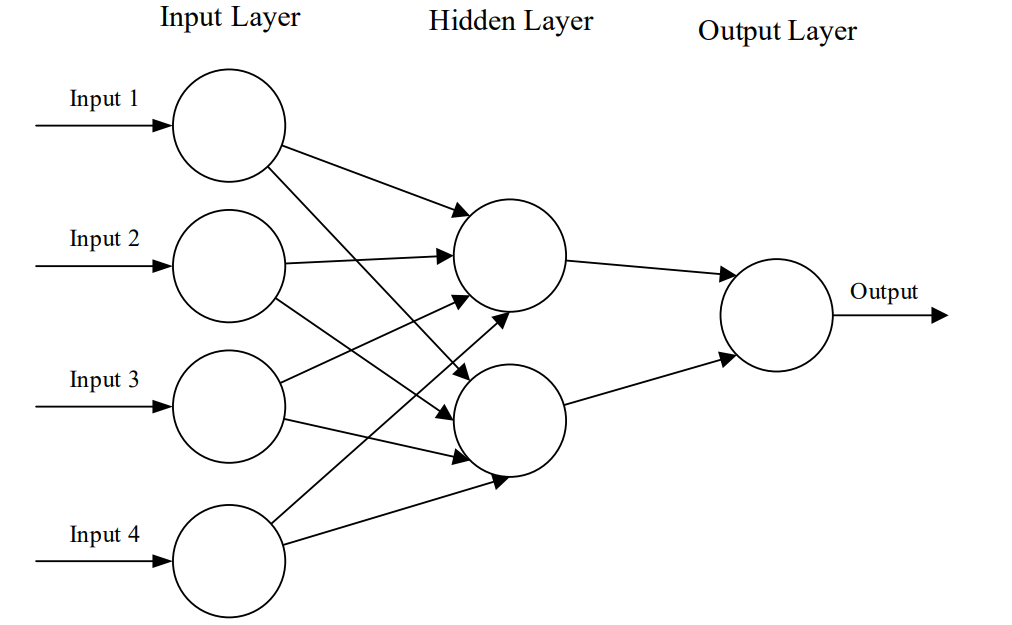
\includegraphics[width=11cm]{figure_ffn.png}
	\caption{Darstellung eines einfachen neuronalen Netzes \parencite{oshea2015cnnintro}.}
	\label{fig:ffn}
\end{figure}

% Einzelnes Neuron im Detail
Die einzelnen Neuronen, auf dem diese Netze aufbauen, sind eine mathematische Modellierung des biologischen Neurons, das erstmals 1943 von Warren McCulloh und Walter Pitts vorgestellt wurde \parencite{Zhou2021machinelearning}. Jedes Neuron empfängt eine Reihe von Eingaben $x_{1 \dots n}$, entweder von externen Quellen oder von den Ausgaben anderer Neuronen. Für jede dieser Eingaben gibt es zugehörige Gewichtungen (engl. \textit{weights}) $w_{1j \dots nj}$, welche die Stärke und Richtung (positiv oder negativ) des Einflusses der jeweiligen Eingaben auf das Neuron bestimmen.

\begin{figure}[h]
	\centering
	\vspace*{4mm}
	%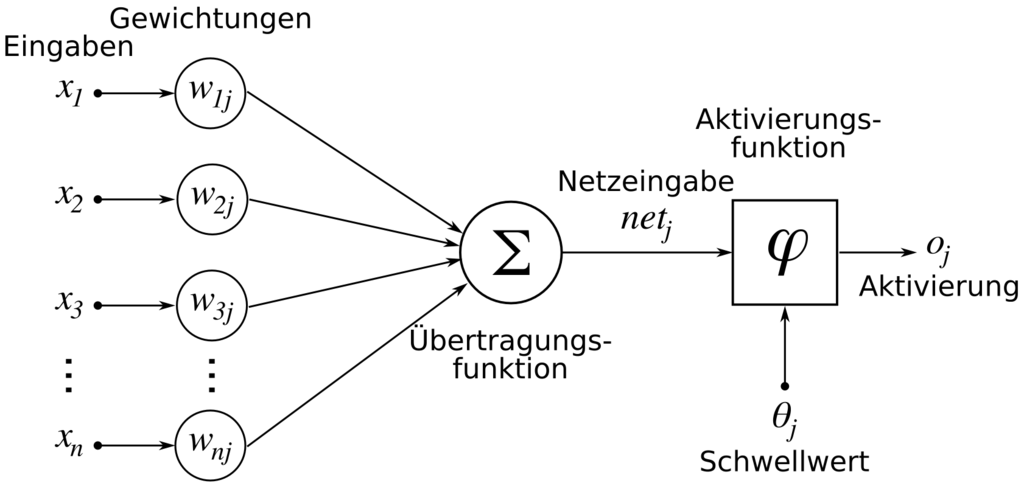
\includegraphics[width=12cm]{figure_mp-neuron.png} % https://commons.wikimedia.org/w/index.php?curid=224561
	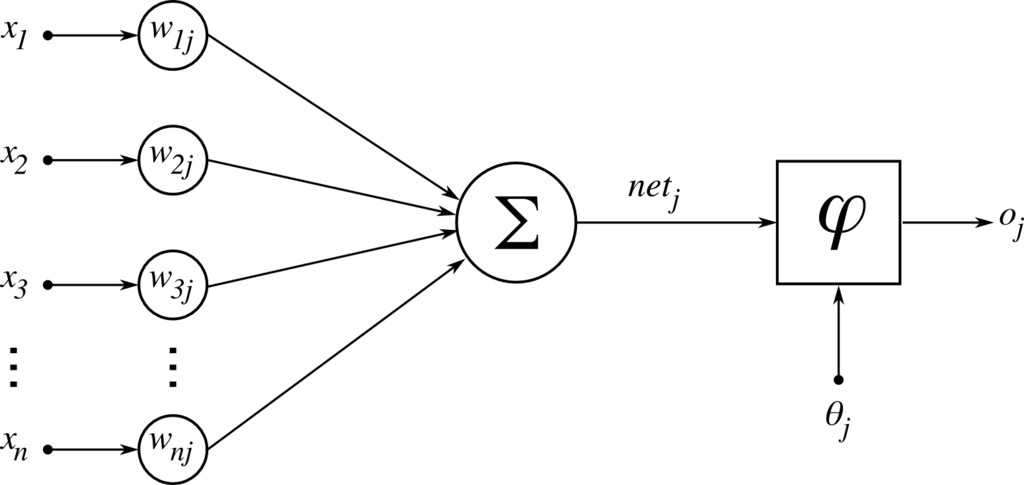
\includegraphics[width=12cm]{figure_mp-neuron_nd.png} % https://commons.wikimedia.org/wiki/File:ArtificialNeuronModel.png
	\vspace*{2mm}
	\caption{Das McCulloch-Pitts-Modell eines Neurons.}
	\label{fig:neuron}
\end{figure}

% Aktivierung allgemein
Das Neuron berechnet dann die gewichtete Summe aller Eingaben und falls ein bestimmter Schwellenwert (engl. \textit{bias}) überschritten wurde, wird das Neuron aktiviert:

\begin{equation}
	o_j = \phi \left( \sum_{i=1}^{n} w_i x_i - \theta_j \right)
	\label{eq:mp-neuron}
\end{equation}

% Aktivierungsfunktionen; Sigmoid & Softmax
Die Aktivierungsfunktion $\phi$ kann dabei unterschiedlich gewählt werden, um die Ausgabe des Neurons zu modellieren. Eine simples Beispiel ist die sogenannte Schwellenwertfunktion (engl. \textit{step function}), die den Wert 1 zurückgibt, wenn die gewichtete Summe größer als der Schwellenwert ist, sonst 0. Eine häufig verwendete Aktivierungsfunktion ist jedoch die sogenannte Sigmoid-Funktion, die kontinuierlich und differenzierbar ist und somit die Optimierung des Netzwerks vereinfacht:

\begin{equation}
	\text{Sigmoid}(x) = \frac{1}{1 + e^{-x}}
	\label{eq:sigmoid}
\end{equation}

Während die Sigmoid-Funktion allerdings nur für binäre Klassifikationen geeignet ist, wird für die Klassifikation von mehreren Klassen die Softmax-Funktion verwendet, die die Wahrscheinlichkeitsverteilung über alle Klassen berechnet:

\begin{equation}
	\text{Softmax}(x)_i = \frac{e^{x_i}}{\sum_{j=1}^{n} e^{x_j}}
	\label{eq:softmax}
\end{equation}

% Wie neuronale Netze lernen; Loss-Funktionen, Backpropagation, Stochastic Gradient Descent
Im Training fließen die Eingabedaten in einer Vorwärtsausbreitung (engl. \textit{forward propagation}) durch das Netzwerk, um die Ausgabe zu berechnen. Es wird dann eine geeignete Verlustfunktion (engl. \textit{loss function}) angewendet, um den Fehler des Modells zu berechnen. Das Ziel des Trainings ist es, die Gewichtungen der Neuronen so anzupassen, dass der Fehler minimiert wird.

Diese Optimierung geschieht durch eine Rückwärtsausbreitung (engl. \textit{backpropagation}), welche den berechneten Fehler rückwärts durch das Netz propagiert, um die Gewichte und Schwellenwerte um einen geringen Wert in die Richtung anzupassen, die den Fehler minimieren würde. Dieser Prozess wird in der Regel mit dem Stochastic Gradient Descent (SGD) Algorithmus durchgeführt, der die Gewichtungen iterativ anpasst, um den Fehler zu minimieren.

% Outro; Vielseitigkeit, Anwendungsbereiche

\subsection{Out-of-Distribution Daten} \label{sec:ood}

% Definition und Problematik
Wenn ein KI-Modell mit Daten konfrontiert wird, die außerhalb des Bereichs liegen, den es während des Trainings gesehen hat, spricht man von Out-of-Distribution (OOD) Daten. Es handelt sich also um Datenpunkte oder Muster, die sich signifikant von den Trainingsdaten unterscheiden. Dies kann zu Problemen führen, da das Modell möglicherweise nicht in der Lage ist, angemessene Vorhersagen oder Entscheidungen für diese Daten zu treffen. Stattdessen werden falsche Vorhersagen mit übermäßigem Vertrauen getroffen.

% OOD-Detection
Die Erkennung von OOD-Daten ist ein wichtiges Forschungsgebiet im maschinellen Lernen, da sie dazu beitragen kann, die Zuverlässigkeit und Sicherheit von KI-Systemen zu verbessern. Idealerweise sollte ein neuronales Netz höhere Softmax-Wahrscheinlichkeiten für In-Distribution-Daten und niedrigere Wahrscheinlichkeiten für OOD-Daten ausgeben. Durch Festlegen eines Schwellenwerts für diese Wahrscheinlichkeiten können Instanzen unterhalb des Schwellenwerts frühzeitig als OOD-Instanzen erkannt und entsprechend behandelt werden. In der Praxis kommt dieser Ansatz jedoch oft an seine Grenzen, da die Softmax-Wahrscheinlichkeiten nicht immer zuverlässig sind und das Modell auch für OOD-Daten hohe Wahrscheinlichkeiten ausgeben kann. Daher werden alternative Ansätze verwendet, wie etwa das Training eines binären Klassifikationsmodells zur Unterscheidung von In-Distribution und OOD-Daten.

\subsection{Datenaugmentation und Generalisierung} \label{sec:data-augmentation}

% Definition und Zweck
Datenaugmentation ist ein wichtiger Schritt im Training von neuronalen Netzen, insbesondere bei begrenzten Datensätzen. Sie bezieht sich auf die künstliche Erweiterung des Trainingsdatensatzes durch Anwenden von Transformationen auf die vorhandenen Daten. Diese Transformationen können z.B. Rotation, Skalierung, Verschiebung, Spiegelung, Helligkeitsanpassung oder Rauschen sein. Das Ziel der Datenaugmentation ist es, das Modell robuster gegenüber Variationen in den Eingabedaten zu machen und die Generalisierungsfähigkeit zu verbessern.

% Beispiele
\begin{figure}[h]
	\centering
	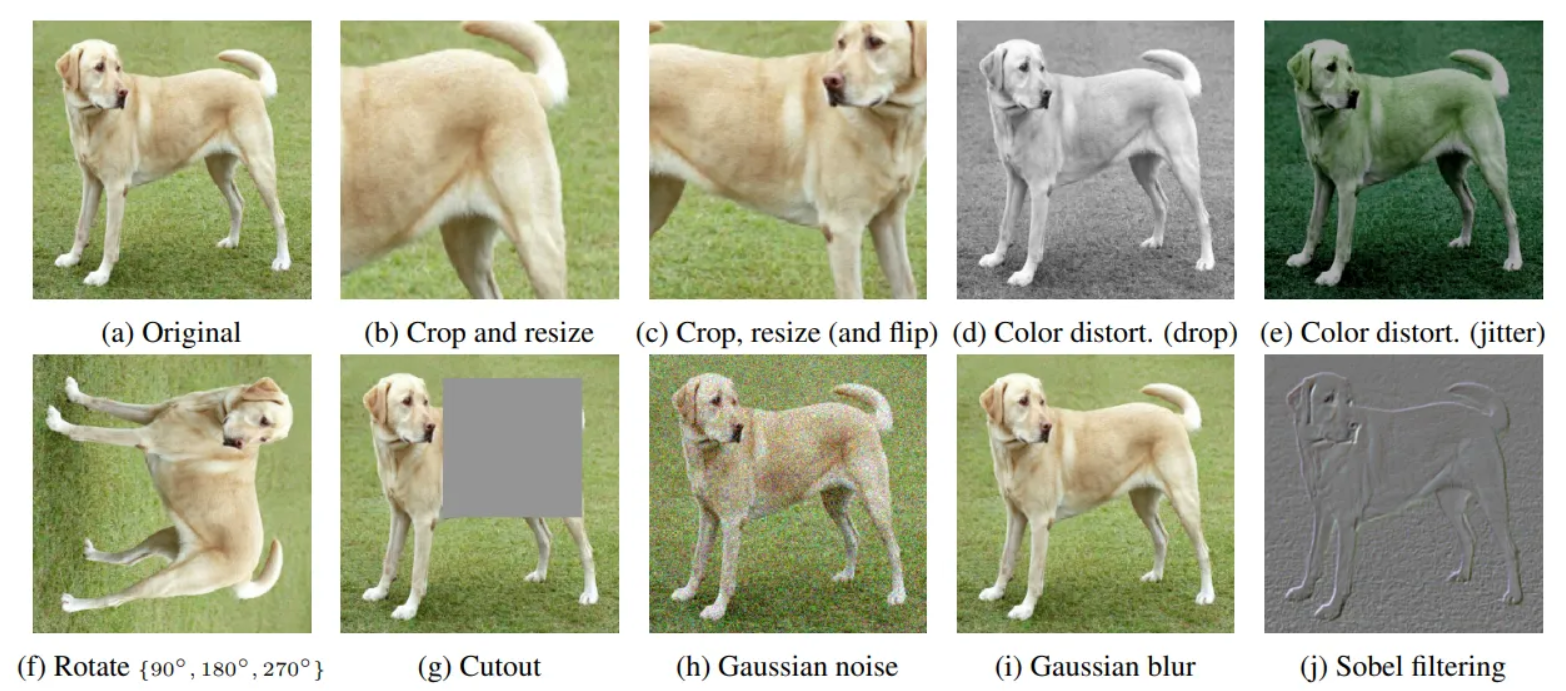
\includegraphics[width=16cm]{figure_data_augmentation.png}
	\caption{Beispiele für unterschiedliche Datenaugmentationstechniken und Kombinationen. \parencite{}} % https://medium.com/lunit/photometric-data-augmentation-in-projection-radiography-bed3ae9f55c3
\end{figure}

\section{Synthetische Daten} \label{sec:synt-data}

% Anschließend an Datenaugmentation; Problematik der Datensammlung

% Abgrenzung synthetischer Datengenerierung zu Datenaugmentation

% (Vorteile und Herausforderungen synthetischer Daten)

% Fortschritte generativer Modellierung, Einleitung folgender Abschnitte

Während die Verfügbarkeit großer Datensätze für das Training von neuronalen Netzen ein entscheidender Faktor für den Erfolg von Deep Learning-Modellen ist, ist es oft schwierig, solche Datensätze zu sammeln, insbesondere in Domänen wie der Medizin oder der Robotik, wo die Daten rar und teuer sind \parencite{}. In solchen Fällen können synthetische Daten eine nützliche Alternative oder Ergänzung zu echten Daten sein.

Synthetische Daten sind künstlich erzeugte Daten, welche die zugrundeliegenden Muster der realen Daten nachahmen. Sie können durch Simulation, Generierung oder Transformation von echten Daten erstellt werden.

...

\subsection{Variational Autoencoder} \label{sec:vae}

Ein Autoencoder ist eine spezielle Art von KI-Modell, das darauf ausgelegt ist, Daten effizient zu komprimieren und dann wieder zu rekonstruieren. Es besteht aus zwei Hauptkomponenten: \parencite{Foster2020gendeeplearning}

\begin{itemize}
	\item einem \textbf{Encoder}-Netzwerk, das hochdimensionale Eingabedaten in einem niederdimensionalen Darstellungsvektor komprimiert, und
	\item einem \textbf{Decoder}-Netzwerk, das einen gegebenen Darstellungsvektor zurück in den ursprünglichen hochdimensionalen Raum umwandelt
\end{itemize}

Der Darstellungsvektor ist eine Kompression des Originalbilds in einen niedriger dimensionalen latenten Raum, wodurch es sich beim Autoencoder um eine Form des \textit{Representation Learning} handelt.

Das Training eines Autoencoders erfolgt durch Minimierung des Rekonstruktionsfehlers, der die Differenz zwischen den ursprünglichen Eingabedaten und den rekonstruierten Ausgaben beschreibt. Eine gängige Verlustfunktion hierfür ist der \textit{Mean Squared Error} (MSE):

\begin{equation}
	Loss=\frac{1}{n}\sum_{i=1}^n (x_i-\hat{x}_i)^2
	\label{eq:loss-mse}
\end{equation}

Ein besonders interessantes Versprechen des Autoencoders ist, dass man theoretisch durch die Wahl eines beliebigen Punkts im latenten Raum neue Bilder erzeugen kann, indem man diesen Punkt durch den Decoder schickt, da der Decoder gelernt hat, wie man Punkte im latenten Raum in realistische Bilder umwandelt. \parencite{Foster2020gendeeplearning} In der herkömmlichen Form hat der Autoencoder in Bezug auf diese Aufgabe allerdings einige Schwachstellen.

Der \textbf{Variational Autoencoder} (VAE) adressiert diese Schwachstellen und verwendet probabilistische Methoden, um die Datenverteilung im latenten Raum zu modellieren; Anstatt einen einzelnen, festen Punkt im latenten Raum für jede Eingabe zu lernen, wird eine Verteilung gelernt, aus der die latenten Variablen für jede Eingabe stammen. Dadurch entsteht ein strukturierteer und kontinuierlicher latenter Raum, der es ermöglicht, neue, realistische Daten zu generieren. % \parencite{Kingma2013}?

...

\subsection{Generative Adversarial Networks} \label{sec:gan}

Ein Generative Adversarial Network (GAN) ist ein KI-Modell, das in \parencite{} vorgestellt wurde. GANs bestehen aus zwei neuralen Netzwerken, die gegeneinander antreten, um realistische synthetische Daten zu erzeugen. Diese Technologie hat sich als äußerst mächtig in der Bild- und Datengenerierung erwiesen.

\begin{figure}[h]
	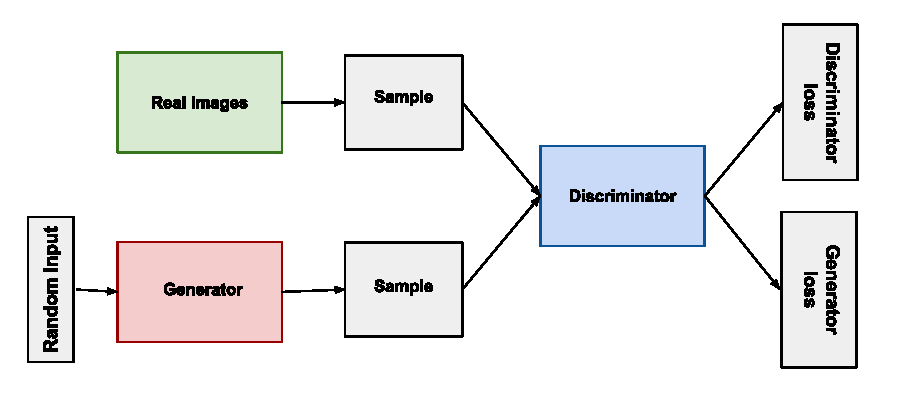
\includegraphics{figure_gan.pdf}
	\caption{Überblick über die GAN-Struktur. Quelle: Google for Developers}
	\label{fig:gan}
\end{figure}

Die Architektur eines GANs besteht aus zwei Hauptkomponenten:

\begin{itemize}
	\item \textbf{Generator}: Das generative Netzwerk nimmt Zufallsrauschen als Eingabe und erzeugt daraus Daten, die möglichst realistisch wirken sollen. Der Generator versucht, die wahre Datenverteilung zu imitieren und realistische Beispiele zu erstellen.
	\item \textbf{Diskriminator}: Das diskriminative Netzwerk erhält sowohl echte Daten aus dem Trainingsdatensatz als auch die vom Generator erzeugten Daten. Seine Aufgabe ist es, zwischen echten und künstlichen Daten zu unterscheiden. Der Diskriminator gibt eine Wahrscheinlichkeit aus, dass die Eingabedaten echt sind.
\end{itemize}

Der Trainingsprozess eines GANs ist als minimax-Spiel zwischen dem Generator und dem Diskriminator formuliert:

\begin{enumerate}[]
	\item \textbf{Diskriminator-Training}: Der Diskriminator wird trainiert, um echte Daten von generierten Daten zu unterscheiden. Dies geschieht durch eine binäre Klassifikation („echt“ oder „synthetisch“). Der Diskriminator passt seine Gewichte an, um die Unterscheidung zu verbessern.
	\item \textbf{Generator-Training}: Der Generator wird trainiert, um den Diskriminator zu täuschen. Dies geschieht, indem der Generator seine erzeugten Daten durch den Diskriminator laufen lässt und die Rückmeldung (Gradienten) des Diskriminators verwendet, um seine eigenen Parameter zu optimieren. Ziel ist es, den Diskriminator zu überlisten, sodass er die generierten Daten als echt klassifiziert.
\end{enumerate}

% Hohe Qualität
% Felixibilität bei Eingangsdaten
% Aber instabiles Training
% Modus-Kollaps
% Hoher Rechenaufwand
...

\subsection{Diffusion Models} \label{sec:diffusion}

% Einleitung
In den letzten Jahren haben sogenannte Diffusion Models für einen enormen Sprung in der Bildgenerierung, insbesondere der Text-to-Image (T2I) Generierung, gesorgt. Das Konzept der Diffusion soll hier deshalb einmal genauer erläutert werden.

% Konzept der Diffusion
Unter Diffusion versteht man den Prozess der langsamen Vermischung von Partikeln oder Informationen über die Zeit. So beschreibt die Diffusionsgleichung in der Physik die zeitliche Entwicklung der Dichte von Teilchen, die sich zufällig bewegen. Im maschinellen Lernen fand das Konzept erstmals in \parencite{} Anwendung. Es entstand eine neue Klasse von generativen Deep Learning-Modellen, die Diffusion Models, welche im Trainingsprozess schrittweise die Struktur der Eingabedaten durch das Hinzufügen von Rauschen auflösen und anschließend darauf trainiert werden, das ursprüngliche Bild aus dem verrauschten Bild zu rekonstruieren.

% Vorwärts- und Rückwärtsdiffusion als Markov-Ketten
Das Training von Diffusion Models teilt sich somit in zwei Phasen auf, die Vorwärts- und die Rückwärtsdiffusion. Beide Phasen ...

\begin{equation}
	q \left( x^{(0 \dots T)} \right) = q \left(x^{(0)}\right)\prod_{t=1}^T q \left(x^{(t)}|x^{(t-1)}\right)
	\label{eq:forward-diffusion}
\end{equation}

In der Rückwärtsdiffusion geht das Bild durch ein Modell, welches selbst nur Rauschen generiert. Es ist die Vorhersage darüber, welches Rauschen vom Eingang entfernt werden soll, um das gewünschte entrauschte Bild zu erhalten.

\begin{equation}
	p \left( x^{(0 \dots T)} \right) = p \left(x^{(T)}\right)\prod_{t=1}^T p \left(x^{(t-1)}|x^{(t)}\right)
	\label{eq:reverse-diffusion}
\end{equation}

Anders als bei GANs gibt es keine direkten adversarialen Optimierungsmechanismen, die zu einem Ungleichgewicht führen können. Es wird stattdessen explizit die Wahrscheinlichkeitsdichte zwischen den realen Daten und den erzeugten Daten minimiert, was zu einem robusteren und stabileren Trainingsprozess führt.

% DALL-E für Text-to-Image
Eine entscheidende Weiterentwicklung der Diffusion Models war die Text-Konditionierung des generativen Prozesses. In \parencite{} wurde DALL-E vorgestellt, ein Modell, das es ermöglicht, Bilder aus Textbeschreibungen zu generieren. DALL-E ...

% Stable Diffusion
...

\section{Semantische Datenaugmentation mit DA-Fusion} \label{sec:da-fusion}

% Einleitung; Kurze Beschreibung, Versprechen der Methode
In \parencite{Trabucco2023dafusion} wird DA-Fusion, eine flexible, auf Stable Diffusion basierende Methode zur Datenaugmentation vorgestellt, die für diese Arbeit von besonderem Interesse ist. Der traditionelle Ansatz der Datenaugmentation, wie in Abschnitt \ref{subsec-data-augmentation} beschrieben, hat sich als effektiv erwiesen, um die Generalisierungsfähigkeit von Modellen zu verbessern. Allerdings erfordert dieser Ansatz auch eine gute Intuition in Bezug auf den verwendeten Datensatz, um zu vermeiden, dass Transformationen gewählt werden, durch die Informationen verloren gehen, die für die Aufgabe des zu trainierenden Modells wichtig sind. Wenn beispielsweise Farbinformationen für die Klassifizierung von Blumen wichtig sind, könnte die Datenaugmentation durch zufällige Farbänderungen die Leistung des Modells verschlechtern. Ein weiteres Beispiel sind Objekte, die klein im Bild sind und durch zufällige Ausschnitte des Bildes aus der Sicht des Modells verschwinden können. DA-Fusion hingegen nutzt das Wissen eines vortrainierten Diffusion Models, um den Bildinhalt semantisch zu verstehen und automatisch neue, realistische Variationen zu generieren.

\begin{figure}[h]
	\centering
	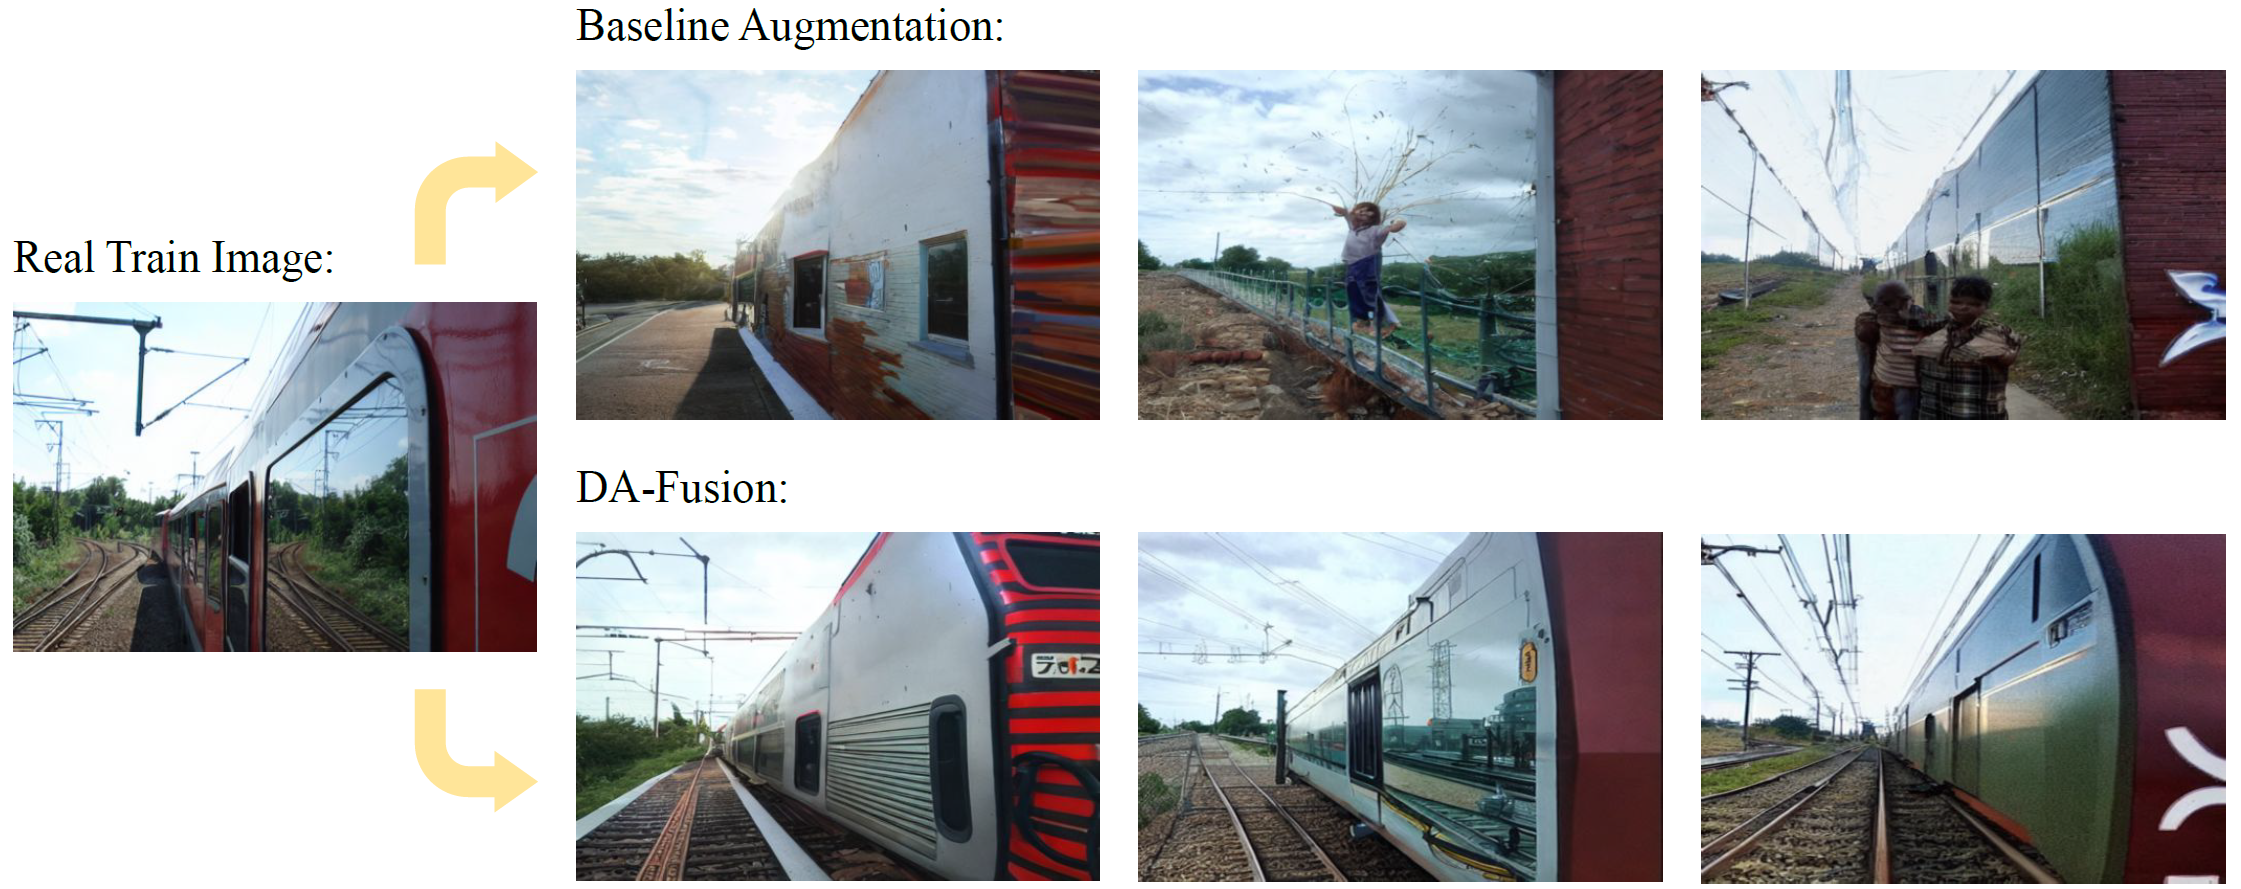
\includegraphics[width=16cm]{figure_da-fusion.png}
	\caption{Vergleich zwischen semantischen Augmentationen aus Baseline-Methode und DA-Fusion \parencite{Trabucco2023dafusion}.}
	\label{fig:da-fusion}
\end{figure}

% Fine-tuning des SD-Modells
Es wird zunächst die Methode Textual Inversion \parencite{} angewendet, um ein vortrainiertes Stable Diffusion-Modell auf den gegebenen Datensatz feinabzustimmen. Dazu wird für jedes neue Konzept bzw. für jede neue Klasse ein Pseudo-Token $y$ in das Modell integriert, der unter Verwendung von Trainings-Prompts wie "a photo of a <$y$>" und den zugehörigen Bilddaten trainiert wird.

% Prozess der Datengenerierung
Anschließend können aus den echten Bildern neue Augmentationen generiert werden, indem den Bildern eine geringe Menge an Rauschen hinzugefügt wird, welches dann wieder durch das feinabgestimmte Modell entfernt werden soll. Hier kommen wieder die selben Text-Prompts zum Einsatz. Auf diese Weise bleibt die grundlegende Struktur der Bilder erhalten, während gleichzeitig neue, semantisch sinnvolle Variationen und Details erzeugt werden.

% Insertion Timestep als Parameter
Ein Vorteil von DA-Fusion ist die Möglichkeit, den Grad der Augmentation durch die Wahl des Insertion Timesteps zu steuern. Der Insertion Timestep bestimmt, wie weit in den Diffusionsprozess das Bild eingefügt wird und wie stark es dafür vorher verrauscht werden muss. Ein niedriger Timestep führt zu stärkeren Augmentationen, während ein hoher Timestep subtilere Variationen erzeugt.

% DA-Fusion schlägt Prompt-Engineering (Real Guidance) für fine-grained Konzepte, auf die das Diffusion-Modell voraussichtlich noch nicht trainiert wurde

% Ein paar Details zur Implementierung

\section{Robuste Datenrepräsentation durch Contrastive Learning} \label{sec:contrastive-learning}

% Einleitung; Themenwechsel abfedern
Neben den vorgestellten Methoden zur Vervielfältigung der Trainingsdaten soll nun auch das Contrastive Learning als effektive Methode zur Verbesserung der Generalisierungsfähigkeit und Robustheit von Modellen vorgestellt werden. Die Methode zielt darauf ab, ähnliche Beispiele im Datensatz zu gruppieren und unähnliche Beispiele voneinander zu trennen. Durch die Kontrastierung der Daten wird eine Art von Supervision erzeugt, die es dem Modell ermöglicht, nützliche Repräsentationen der Eingabedaten zu lernen.

% Eine vielversprechende Alternative zum überwachten Lernen
Contrastive Learning kommt ursprünglich aus dem unüberwachten Lernen. Da die Annotation von Daten sehr aufwendig sein kann, insbesondere in Domänen, in denen Expertenwissen erforderlich ist, hat sich das Contrastive Learning als vielversprechende Alternative mit äußerst starker Generalisierungsfähigkeit und Robustheit gegenüber Adversarial Attacks erwiesen \parencite{Liu2021understandimprovecontrastivelearning}.

% Vermehrt auch überwachte Methoden; *Class* statt *Instance* Discrimination (Keshtmand2022)
Mittlerweile gibt es vermehrt Ansätze, Contrastive Learning auch im überwachten Setting anzuwenden, um die Repräsentationen von Daten zu verbessern. Während das Modell im unüberwachten Setting lernt, zwischen einzelnen Instanzen zu unterscheiden, werden im überwachten Setting die Klassenzugehörigkeit der Beispiele berücksichtigt.

% Folgende Abschnitte
In den folgenden Abschnitten wird genauer auf die Funktionsweise von sowohl unüberwachten als auch überwachten Varianten des Contrastive Learning eingegangen, die in den letzten Jahren vielversprechende Ergebnisse erzielt haben.

\subsection{Unsupervised Contrastive Learning} \label{sec:unsup-contrastive}

% Grundprinzipien, Funktionsweise (im Detail, technisch)
Ob unüberwacht oder überwacht: Im Contrastive Learning soll die Distanz ähnlicher Beispiele in einem Repräsentationsraum minimiert und die Distanz unähnlicher Beispiele maximiert werden. Dazu bildet das Modell kontrastive Paare aus einem Anchor-Beispiel und verschiedenen positiv- oder negativ-Beispielen. Je nach Methode kann vor allem die Anzahl der positiv- und negativ-Beispiele pro Anchor variieren, wodurch sich auch die jeweiligen Loss-Funktionen unterscheiden.

% SimCLR (Chen2020) als prominentes Beispiel
	% NT-Xent Loss (Normalized Temperature-scaled Cross-Entropy Loss)
		% Ganzer Batch statt Triplet o.Ä.
		% Jeder Anchor 2x augmentiert (2 Ansichten): ergibt positives Paar, alle anderen Beispiele im Batch sind negative Beispiele
		% CNN als Feature Extractor: encodiert die Eingabedaten in eine hochdimensionale Repräsentation
		% Projection Head: transformiert die features weiter, um einen Repräsentationsraum zu erzeugen, der für die Unterscheidung der Beispiele geeignet ist
			% 2-Layer MLP mit ReLU-Aktivierung
		% Similarity Scores: Cosine Similarity zwischen den Repräsentationen der Beispiele
		% Softmax über die Scores aller Paare im Batch, mit Temperature Scaling, um die Unterscheidung zwischen positiven und negativen Paaren hervorzuheben
	% Aggressive Data Augmentation (aus der die 2 Ansichten entstehen) entscheidend, um die Robustheit der Repräsentationen zu verbessern
	% Größere Batch Sizes und längere Trainingszeiten begünstigen die Lernfähigkeit des Modells
	% Zudem sind Hard Negatives entscheidend für den Erfolg des Modells
Das wohl prominenteste Beispiel für Contrastive Learning ist \textbf{SimCLR}, das in \parencite{Chen2020simclr} vorgestellt wurde. SimCLR verwendet den NT-Xent Loss (Normalized Temperature-scaled Cross-Entropy Loss), der die Ähnlichkeiten zwischen allen Paaren im Batch (auch \textit{Mini-Batch}) berücksichtigt, anstatt nur einzelne Triplets oder Paare. Jedes Beispiel wird dabei zweimal augmentiert, um zwei Ansichten zu erzeugen, welche als positives Paar für das jeweilige Beispiel dienen. Alle anderen Beispiele (bzw. dessen Ansichten) im Batch werden als negativ-Beispiele gesehen.

Die Eingabedaten werden durch ein Convolutional Neural Network (CNN) in eine hochdimensionale Repräsentation transformiert. Dieser Schritt wird auch als \textit{Feature Extraction} bezeichnet. SimCLR verwendet anschließend einen sogenannten \textit{Projection Head}, der die encodierten Repräsentationen weiter transformiert, um einen Repräsentationsraum zu erzeugen, der für die Unterscheidung der Beispiele geeignet ist. In diesem Representationsraum werden die Ähnlichkeitswerte der Paare berechnet, um den Loss zu bestimmen.

Dafür wird die Kosinus-Ähnlichkeit $s_{i,j}$ der Paare $z_i$ und $z_j$ berechnet:

\begin{equation}
	s_{i,j} = \frac{z_i \cdot z_j}{\|z_i\| \cdot \|z_j\|}
	\label{eq:cosine-similarity}
\end{equation}

Der Loss ergibt sich dann aus der Berechnung des Softmax über die Ähnlichkeiten aller Paare im Batch, skaliert mit einem Temperaturparameter, um die Unterscheidung zwischen positiven und negativen Paaren hervorzuheben.

Durch die Verwendung aggressiver Datenaugmentation zur Erzeugung der zwei Ansichten wird die Robustheit der Repräsentationen verbessert. Größere Batch Sizes und längere Trainingszeiten begünstigen die Lernfähigkeit des Modells. Besonders die Wahl von \textit{Hard Negatives}, also von Paaren, welche ähnliche Konzepte darstellen, aber sehr unterschiedlich aussehen, hat sich als entscheidend für den Erfolg des Modells erwiesen.

% Eine neuere Variante: StableRep (Tian2023)
	% Verwendung von synthetischen Daten aus T2I-Modellen, insbesondere Stable Diffusion
	% Verwendet Bilder, die aus dem selben Prompt generiert wurden, als positive Beispiele voneinander
	% Kann mit den richtigen Einstellungen auch mit Training nur auf synthetischen Daten die Leistung von SimCLR übertreffen
	% Noch bessere Ergebnisse bei Einbeziehung von Textsupervision

\subsection{Supervised Contrastive Learning} \label{sec:sup-contrastive}

% Erweiterung der Contrastive Learning-Methode durch Verwendung von Label-Informationen

% SupCon (Khosla2020)
	% Weiterentwicklung der Loss-Funktion, die mehrere positiv-Beispiele pro Anchor-Sample berücksichtigt und das Contrastive Learning auf das Supervised Setting anpasst
	% Eine rein naive Anpassung wird aber um einige wünschenswerte Anpassungen erweitert
		% Es wird nicht ein Anchor, ein positiv-Beispiel und viele negativ-Beispiele verwendet; stattdessen kommen im Supervised Contrastive Learning auch viele positiv-Beispiele pro Batch zum Einsatz
		% Die *vielen* positiv-Beispiele werden zudem nicht mehr als Augmentationen des Anchor-Samples generiert, sondern als Samples der gleichen Klasse herangezogen
		% So soll auch die Notwendigkeit des Hard-Negative Minings reduziert werden
		% Trotzdem wird gezeigt, dass der resultierende Loss sowohl von hard-negatives wie auch hard-positives profitiert
		% Verwendung des Mittelwertes der positiven Repräsentationen stabilisiert das Training und führt zu einer verbesserten Leistung

% Generalized SCL (Kim2022)
	% Label als Distribution

% Supervised Contrastive Learning with Hard Negatives (Jiang2022)
	% Zusätzliche Einschränkung des Negative Samplings für Auswahl von Hard Negatives (Nähe im Repräsentationsraums)
...

\section{Forschungslücke} \label{sec:research-gap}

% Rückverweis auf Anwendungsfall

% Einleitung für den vorzustellenden Ansatz
...

\subsection{Herausforderungen bei der Generierung synthetischer Daten} \label{sec:challenges-synt-data}

% Herausforderungen bei der Generierung synthetischer Daten
	% Komplexe Objekte
	% Feine Unterschiede zwischen Klassen
	% Wenig Variation
	% (Detaillierte Meta-Informationen, Multimodalität)
	% Risiko der Fehlklassifikation von OOD-Daten

% Welche Anforderungen ergeben sich?
	% Hohe Kontrolle über die Generierung der synthetischen Daten; Genauigkeit
	% Trotzdem Verbesserung der Generalisierungsfähigkeit
	% Verbesserung der OOD-Detektion
...

\subsection{Synthetische Daten als negativ-Beispiele im Contrastive Learning} \label{sec:synt-ood-contrastive}

% Anschließend an die Herausforderungen bei der Datengenerierung
% Frage: Könnte Contrastive Learning eine Möglichkeit bieten, auch aus mangelhaften Daten zu lernen?
	% Dürfen nicht zu entfernt sein: CL lernt vor allem aus HARD Negatives
		% SimCLR profitierte besonders von hard negatives, um gute Repräsentationen zu lernen
	% Sind NEAR OOD-Daten gute Hard Negatives?
		% Gilt es, zu untersuchen
		% Near OOD-Negatives sind nah genug an den echten Daten, um die Repräsentationen zu verbessern, aber dennoch OOD genug, um die Distanz zu maximieren
% Forschungslücke; Was wurde schon untersucht? Wo ist die Lücke?
	% StableRep: Synthetische Diffusion-Daten im Contrastive Learning, aber nur normale ID-Beispiele
		% Stable Diffusion "off-the-shelf" ist nicht akkurat genug
			% Objekte zu komplex
			% Zu ähnlich; feine Unterschiede
		% Auch die gleichbleibenden Hintergründe sind fatal
		% Außerdem: Unsupervised
	% SCL mit Hard Negatives: Verfeinertes Negative Sampling, aber ohne synthetische Daten
		% Gute Strategie für Negative-Sampling
		% Aber keine synthetischen Daten
	% Was wenn: Anstatt Negatives aus Nähe im Darstellungsraum zu samplen, Near OOD-Augmentationen aus Anchor-Klasse?
...

\subsection{Integration von DA-Fusion und Supervised Contrastive Learning} \label{sec:da-fusion-scl}

% DA-Fusion zur Generierung von ID- und Near OOD-Daten
% Einfach den strength-Parameter der DA-Fusion-Augmentationen erhöhen
% Bei der Generierung die Maske verwenden, damit die Hintergründe gleich bleiben
% Supervised Contrastive Learning mit eigener Sampling-Strategie für Near OOD-Negatives

% Potenzielle Vorteile
	% Bessere Generalisierung trotz Limitationen in der Datengenerierung
		% OOD-Augmentationen müssen an sich keine spezifischen Klassen akkurat repräsentieren, sind aber dennoch nah genug an den echten Daten, um dessen Repräsentationen zu verbessern
	% Bessere OOD-Detektion
		% OOD-Detection profitiert von einer guten Repräsentation der Daten, um die Distanz zwischen In-Distribution und OOD-Daten zu maximieren
% Potenzielle Herausforderungen
	% ...
...